  \documentclass[
    a4paper,
    abstracton,
    twocolumn,
    emulatestandardclasses
  ]{scrartcl}

  \usepackage[english]{babel}
  \usepackage{xcolor}
  \usepackage{authblk}
  \usepackage{amsthm}
  \usepackage{amsmath}
  \usepackage{amssymb}
  \usepackage{physics}
  \usepackage{csquotes}
  \usepackage{paralist}
  \usepackage[
    backend=biber,
    sorting=none
  ]{biblatex}
  \usepackage{graphicx}
  \usepackage[hidelinks]{hyperref}
  \usepackage{cleveref}
  \usepackage[binary-units]{siunitx}
  \usepackage[
    margin=10pt,
    labelfont=bf
  ]{caption}
  \usepackage{booktabs}
  \usepackage{pgfplots}
  \usepackage{adjustbox}
  \usepackage[acronym]{glossaries}

  \title{MRI to CT Translation with GANs}
  \author[1]{Bodo Kaiser}
\author[2]{Shadi Albarqouni}
\affil[1]{\textit{bodo.kaiser@physik.uni-muenchen.de}}
\affil[2]{\textit{shadi.albarqouni@tum.de}}

\pgfplotsset{compat=newest}
\addbibresource{literature.bib}

\newacronym{ct}{CT}{X-ray computed tomography}
\newacronym{mri}{MRI}{magnetic resonance imaging}
\newacronym{pd}{PD}{proton density}
\newacronym{t1}{T1}{spin-lattice relaxation time}
\newacronym{t2}{T2}{spin-spin relaxation time}
\newacronym{mp}{MP}{magnetization-prepared}
\newacronym{itk}{ITK}{Insight Segmentation and Registration Toolkit}
\newacronym{rage}{RAGE}{RF pulse and rapid gradient echo}
\newacronym{mhd}{MHD}{MetaImage Header}
\newacronym{pet}{PET}{positron emission tomography}
\newacronym{rire}{RIRE}{Retrospective Image Registration Evaluation}
\newacronym{nifti}{NIfTI}{Neuroimaging Informatics Technology Institute}
\newacronym{oasis}{OASIS}{Open Access Series of Imaging Studies}
\newacronym{adni}{ADNI}{Alzheimer's Disease Neuroimaging Initiative}

\begin{document}

\makeatletter
\twocolumn[
	\begin{@twocolumnfalse} 
		\maketitle
		\begin{abstract}
  We present a detailed description and reference implementation of
  preprocessing steps necessary to prepare the public \gls{rire} dataset
  for the task of \gls{mri} to \gls{ct} translation. Furthermore we describe
  and implement three state of the art \gls{cnn} and \gls{gan} models where
  we report statistics and visual results of two of them.
\end{abstract}

		\vspace{1em}
	\end{@twocolumnfalse}
]
\makeatother

\section{Introduction}

Computer tomography (CT) and magnetic resonance imaging (MR) are the main
workhorses of clinical diagnosis and cancer monitoring as they reveal the
condition of the patients inner organs.

In consequence of CT and MR exploiting distinct physical effects both
modalities take complementary roles inside the present clinical framework
with MR being more the informative and safe~\cite{Hartwig09} but also
more expensive modality.


While CT is based on the interaction of high energy photons (x-rays) with
biological tissue, MR 


, therefore so called image guided planning based on the
patients CT scan is used to estimate the patients specific radiation treatment
planning. Even though x-rays used for imaging are of a lower energy band
as x-rays used for cancer treatment, it has been shown that they still possess
a risk of developing new cancer inside the patient~\cite{Martin06}.
MR on the other hand takes advantage of the magnetic properties of hydrogen
and is not associated with any health risks . Furthermore MR
provides a much higher soft tissue contrast which is useful for cancer
classification. Although MR and CT differ significant in the applied
physics the high entropy in MR data suggests the existence of a one
directional mapping from MR to CT space whereby the acquisition of CT would
become obsolete. Beside the stated health benefits for the patients such an
approach would reduce expanses and also would free CT resources for
emergency cases where the fast acquisition of CT is used to locate internal
bleedings.

\section{Related Work}

Since the early days of \gls{ct}, health manufacturer were attempted to reduce
radiation exposure in \gls{ct} scans by using, for instance, more sensible
detection electronics, and more sophisticated scanning sequences. Through the
growing availability of computing power we also find evermore computer vision
techniques being utilized, for example, in the enhancement of image quality of
low-dose \gls{ct}s~\cite{Xu12}. Altough these efforts have lead to an
impressive and steady evolution of the \gls{ct} apparatus, they still require
the patient to be irradiated nevertheless.
First approaches which dispense the radiation exposure, through the
computational transformation of \gls{mri} to \gls{ct}, relay on the
atlas-based transformations applied to \gls{mri} to predict \gls{ct}, see
Ref.~\cite{Hofmann08}. Further improvements thereto include, for instance,
random forests~\cite{Andreasen13}. Finally it has been shown that these
\gls{ct} prediction methods can in fact already replace physical \gls{ct}
for treatment planning~\cite{Andreasen2017}.
At the same time, we have seen an incredible progress with deep learning
techniques in computer science~\cite{LeCun15}. Recent efforts with \gls{gan}s,
see Ref.~\cite{Goodfellow14}, seem to be a promising path towards finding
a global optimum in training neural networks through the use of game theory.
Furthermore \gls{gan}s proved significant improvements over the former state
of art in the task of image to image translation~\cite{Isola16} but also the
generalization of three dimensional structures inside the so called latent
space~\cite{ZXFT16}.
Keeping this in mind, the medical computer vision community rapidly adapted
\gls{gan}s for their own specific tasks. In comparison to datasets common in
general computer vision, medical datasets typical comprise volumetric single
channel images with high bit depth. Bearing the challenge of \gls{ct} from
\gls{mri} prediction in mind, the expectations towards \gls{gan}s have been
lately shown increased performance to the previous approaches~\cite{Nie16}.
Yet, the full potential of \gls{gan}s have not been exhausted. For example,
it has been shown that \gls{gan}s are capable of being trained with
unregistered modalities~\cite{Wolterink17}.
Beside the enourmous breakthroughs made in medical computer vision we still
see a shortage in a reproducable comparison of recent methods with publicly
available data. Not to mention the open questions with regard to best
practices in choosing good \gls{gan} model parameters for the task of
\gls{ct} prediction which we hope to address in the subsequent sections.

\section{Method}

\subsection{Dataset}

There are several \gls{mri} and \gls{ct} datasets available, for
instance, \gls{oasis}~\cite{OASIS} or \gls{adni}~\cite{ADNI}. Unfortunately
public datasets in which both modalities are obtainable for the same subject
are, to date, rare. To our knowledge only the \gls{rire} project~\cite{RIRE}
and the Cancer Imaging Archive~\cite{CIA} provide \gls{mri} and \gls{ct}
volumes for some subjects. For the present work we limited ourselves to the
data from the \gls{rire} project, as the volumetric data was available in the
same format.
\begin{table}[h]
  \centering
  \begin{tabular}{*{6}{c}}
    \toprule
    & \multicolumn{4}{c}{\acrshort{mri}}
		& \\
   	\cmidrule{2-5}
    \acrshort{ct} &
		\acrshort{pd} &
		\acrshort{t1} &
		\acrshort{t2} &
		\acrshort{mp} \acrshort{rage} &
		\acrshort{pet} \\
    \midrule
    \num{17} & \num{14} & \num{19} & \num{18} & \num{9} & \num{8} \\
             & \num{12} & \num{17} & \num{16} & \num{9} & \num{6} \\
    \bottomrule
  \end{tabular}
  \caption{Subject statistics with respect of the available imaging
    modalities of the \gls{rire} dataset. The second table only accounts for
    subjects with available \gls{ct} data.
  }\label{tab:rire}
\end{table}
In \Cref{tab:rire} we list the aggregated modality count of the \gls{rire}
dataset (first row). As we use the \gls{ct} as target space, we created a
second modality count on the subjects with \gls{ct} modality (second row).
Beside of \gls{ct} one can also obtain \gls{pet} images for some subjects.
Next to the common \gls{t1} and \gls{t2} weighted \gls{mri}, some subjects of
the \gls{rire} dataset also offer \gls{pd} and \gls{mp} \gls{rage} weighted
\gls{mri}s. Some \gls{mri}s can be obtained in a rectified version, which we
did not use. We used the \gls{t1} weighted \gls{mri} together with the
\gls{ct} as input and target data as these give us the highest subject count.
However, it would be an interesting experiment to supply different \gls{mri}s
as multi-channel input.

\subsection{Preprocessing}

The modality data for each subject can be downloaded from the website of the
\gls{rire} project, see Ref.~\cite{RIRE}. In \Cref{fig:conversion} we depicted
the first preprocessing step, that involves the extraction, decompression and
conversion of the downloaded data. After extraction and decompression the
volumetric data presents itself as \gls{mhd}. We converted the \gls{mhd} files
to the self-contained \gls{nifti} format through the Python front-end of the
\gls{itk} library.
\begin{figure}[h]
  \centering
  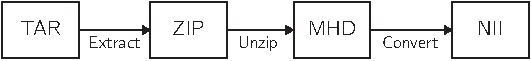
\includegraphics[width=\linewidth]{figure/conversion.pdf}
  \caption{Image extraction and conversion from \gls{mhd} to \gls{nifti}
		format.
	}\label{fig:conversion}
\end{figure}
\Cref{fig:registration} illustrates the coregistration procedure as part of
the image preprocessing. The coregistration yields a rigid transformation that
aligns the moving volume with the fixed volume. In our case it makes sense to
use the \gls{ct} volume as the fixed volume because the \gls{ct} are in
general better centered. Given a rigid transformation, a linear interpolator
returns a translated volume from the sample points of the initial \gls{mri}.
The mutual information between the moved \gls{mri} and the \gls{ct} is then
used to optimize the rigid transformation. The procedure is executed
iteratively and stopped when the maximum iterations steps are reached or
the convergence parameter is met. As the implementation of the interpolator
and transformation optimizer is not a trivial undergoing, therefore we
reverted back to the \gls{itk} library, see Ref.~\cite{Yaniv2018}.
\begin{figure}[h]
  \centering
  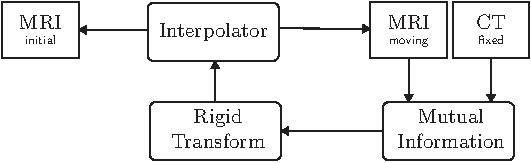
\includegraphics[width=\linewidth]{figure/registration.pdf}
  \caption{Multi-modal image coregistration using maximum mutual information
    optimizer.
	}\label{fig:registration}
\end{figure}
Finally we used a binary fill holes algorithm from SciPy~\cite{SciPy} to
remove the \gls{ct} table present in some \gls{ct} volumes as well as
background noise.\footnote{The complete preprocessing described so far is
available at \url{https://github/bodokaiser/mrtoct-scripts}.}

\subsection{Network}

As generative adversarial networks we decided to use pix2pix~\cite{Isola16}
as it has already shown great results in the task of color image to image
translation and context-aware 3d synthesis~\cite{Nie16} which uses a simpler
generator but accounts for 3d structures.

As convolutional encoder-decoder network we chose u-net~\cite{Ronneberger15}
as it was able to compete with much larger models in the task of semantic
segmentation~\cite{Badrinarayanan15}. Further our implementation of pix2pix
uses u-net as generator network, hence we are able to evaluate the impact
of the adversarial min-max approach.

\subsubsection{u-net}

\begin{figure}[h]
  \centering
  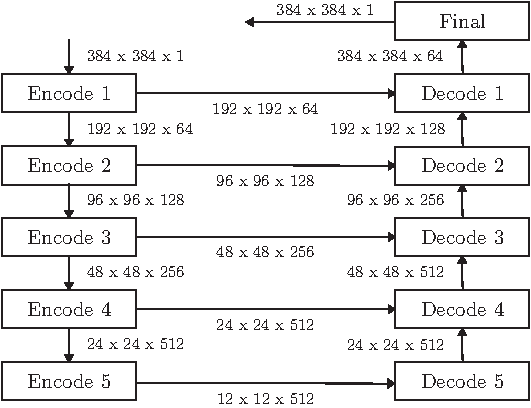
\includegraphics[width=\linewidth]{figure/unet-arch.pdf}
  \caption{The u-net generator architecture.
	}\label{fig:unet:arch}
\end{figure}
\begin{table}[h]
  \centering
  \begin{tabular}{lcccc}
    \toprule
    Block & Kernel & Strides & Padding & Initializer \\
    \midrule
    Encode & \num{4} & \num{2} & Same & Xavier \\
    Decode & \num{4} & \num{2} & Same & Xavier \\
    Final  & \num{3} & \num{2} & Same & Xavier \\
    \bottomrule
  \end{tabular}
  \caption{Convolution parameters used in the u-net blocks.
  }\label{tab:unet:conv}
\end{table}
\begin{figure}[h]
  \centering
  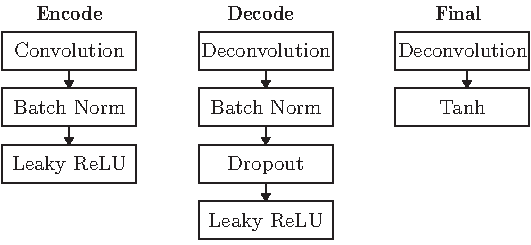
\includegraphics[width=\linewidth]{figure/unet-block.pdf}
  \caption{The u-net encoder, decoder and final block.
	}\label{fig:unet:block}
\end{figure}

\subsubsection{Pix2Pix}

\subsubsection{3D Synthesis}

\subsection{Losses}

\subsubsection{Distance Losses}

As norm losses we refer to the mean absolute error ($L1$ loss) and the
mean squared error ($L2$ loss).

\subsubsection{Gradient Losses}

The gradient (difference) loss is used in the framework of context-aware
3d synthesis~\cite{Nie16} in addition to the norm loss.

\subsubsection{Signal Losses}

From signal processing PSNR,SSE

\subsubsection{Adversarial Loss}

Least-squared adversarial loss, standard adversarial loss. BEGAN loss?


\subsection{Augmentation}

\subsubsection{Random Crop}
\subsubsection{Rotation}
\subsubsection{Contast Adjustment}


\input{section/result}

\clearpage
\printbibliography{}

\end{document}
